\documentclass{article}
\usepackage{amsmath, amssymb, amsthm}
\usepackage{geometry}
\usepackage{graphicx}
\usepackage{tikz}
\geometry{a4paper, margin=1in}
\usepackage{titlesec}
\usepackage{hyperref}
\setcounter{MaxMatrixCols}{20}

\title{Obtaining a Strongly Regular Design by Deleting a Vertex from a Rook Graph}
\author{}
\date{}

\begin{document}

\maketitle
\begin{figure}[h!]
\centering
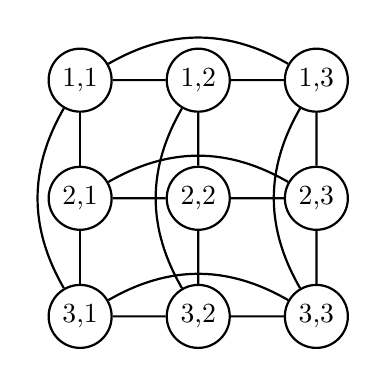
\begin{tikzpicture}[scale=1.5, every node/.style={circle, draw, inner sep=1.5pt, minimum size=0.8cm}, every path/.style={thick}]

% Define coordinates for vertices
\node (v11) at (0, 3) {1,1};
\node (v12) at (1, 3) {1,2};
\node (v13) at (2, 3) {1,3};

\node (v21) at (0, 2) {2,1};
\node (v22) at (1, 2) {2,2};
\node (v23) at (2, 2) {2,3};

\node (v31) at (0, 1) {3,1};
\node (v32) at (1, 1) {3,2};
\node (v33) at (2, 1) {3,3};

% Draw edges for rows
\foreach \i in {1,2,3} {
    \foreach \j [count=\k from 2] in {1,2} {
        \draw (v\i\j) -- (v\i\k);
    }
}

% Draw edges for columns
\foreach \j in {1,2,3} {
    \foreach \i [count=\k from 2] in {1,2} {
        \draw (v\i\j) -- (v\k\j);
    }
}

% Add curved edges to connect the corners
\draw[bend right] (v11) to (v31); % Connect (1,1) to (3,1)
\draw[bend left] (v11) to (v13); % Connect (1,1) to (1,3)
\draw[bend right] (v13) to (v33); % Connect (1,3) to (3,3)
\draw[bend left] (v31) to (v33); % Connect (3,1) to (3,3)

\draw[bend right] (v12) to (v32);
\draw[bend left] (v21) to (v23);

\end{tikzpicture}
\caption{Rook graph \( R_{3,3} \), with vertices labeled as \( (i, j) \) representing the cells of a \( 3 \times 3 \) chessboard. Edges connect vertices in the same row or column.}
\label{fig:rook-graph}
\end{figure}


\begin{abstract}
This paper explores the relationship between rook graphs and strongly regular designs. Specifically, we analyze the structural and algebraic consequences of deleting a single vertex from a rook graph. Using adjacency matrix partitioning and coherent rank, we demonstrate how this operation results in a strongly regular design, resulting in a graph with coherent rank 10.
\end{abstract}

\newpage
\section{Introduction}

Rook graphs, arising naturally from the geometry of a chessboard, provide a fascinating intersection of combinatorics and algebra. These graphs, defined by vertices corresponding to cells and edges connecting vertices in the same row or column, inherit their structure from orthogonal arrays. The inherent symmetry of these graphs leads to rich combinatorial properties.

In this paper, we investigate the effect of deleting a single vertex from a rook graph, a process that leads to the emergence of a strongly regular design. This is demonstrated using adjacency matrix partitioning and the coherent rank framework, which reflects the structural regularity of the graph.

\section{Definition of a Rook Graph}

A rook graph \( R_{n,n} \) is defined as a graph where:
\begin{itemize}
    \item Vertices represent the cells of an \( n \times n \) chessboard.
    \item Two vertices are adjacent if they lie in the same row or column.
\end{itemize}

Alternatively, rook graphs can be constructed using an orthogonal array \( \text{OA}(2, n) \), which has the following properties:
\begin{itemize}
    \item \( \text{OA}(2, n) \) is a \( 2 \times n^2 \) matrix, where each column corresponds to a unique pair \( (x, y) \in \{1, \dots, n\} \times \{1, \dots, n\} \).
    \item For any two rows, every pair of entries appears exactly once in the same column.
\end{itemize}

The vertices of \( R_{n,n} \) correspond to the columns of \( \text{OA}(2, n) \), with edges defined by shared values in any row.

\section{Construction of the Block Graph}

Given \( \text{OA}(2, n) \), the associated block graph \( G = (V, E) \) is constructed as follows:
\begin{itemize}
    \item Each vertex \( v_i \) corresponds to the \( i \)-th column of the orthogonal array, so \( |V| = n^2 \).
    \item Two vertices \( v_i \) and \( v_j \) are adjacent if they share the same value in any row of the array.
\end{itemize}

For example, for \( n = 3 \), the orthogonal array \( \text{OA}(2, 3) \) is:
\[
\begin{bmatrix}
1 & 1 & 1 & 2 & 2 & 2 & 3 & 3 & 3 \\
1 & 2 & 3 & 1 & 2 & 3 & 1 & 2 & 3
\end{bmatrix}.
\]
The corresponding rook graph has 9 vertices and adjacency relations based on shared row values.

\section{Deletion of One Vertex}

Rook graphs are vertex-transitive, so removing any vertex results in an equivalent graph. For simplicity, let \( v_1 \), corresponding to the coordinate \( \begin{pmatrix} 1 \\ 1 \end{pmatrix} \), be removed. 

After removal:
\begin{itemize}
    \item The degree of the \( 2(n-1) \) vertices originally adjacent to \( v_1 \) decreases by 1.
    \item All other vertices retain their original degrees.
\end{itemize}

This operation partitions the vertices into two subsets:
\begin{enumerate}
    \item The \( 2(n-1) \) vertices adjacent to \( v_1 \), corresponding to
    \begin{align*}
        \begin{pmatrix} 1 \\ 2 \end{pmatrix}, \begin{pmatrix} 1 \\ 3 \end{pmatrix},..., \begin{pmatrix} 1 \\ n \end{pmatrix}, \begin{pmatrix} 2 \\ 1 \end{pmatrix}, \begin{pmatrix} 3 \\ 1 \end{pmatrix},..., \begin{pmatrix} n \\ 1 \end{pmatrix} 
    \end{align*}
    \item The remaining \( (n-1)^2 \) vertices, corresponding to
    \begin{align*}
        \begin{pmatrix} 2 \\ 2 \end{pmatrix}, \begin{pmatrix} 2 \\ 3 \end{pmatrix},...,\begin{pmatrix} 2 \\ n \end{pmatrix},\begin{pmatrix} 3 \\ 2 \end{pmatrix}, \begin{pmatrix} 3 \\ 3 \end{pmatrix},...,\begin{pmatrix} 3 \\ n \end{pmatrix},...,\begin{pmatrix} n \\ 2 \end{pmatrix}, \begin{pmatrix} n \\ 3 \end{pmatrix},...,\begin{pmatrix} n \\ n \end{pmatrix}
    \end{align*}
\end{enumerate}

\section{Adjacency Matrix Partitioning}

Reordering the adjacency matrix \( \mathbf{A} \) by grouping the vertices by their degrees after removing \( v_1 \) reveals a block structure:
\[
\mathbf{A} =
\begin{bmatrix}
\mathbf{A}_1 & \mathbf{C} \\
\mathbf{C}^\top & \mathbf{A}_2
\end{bmatrix},
\]
where:
\begin{itemize}
    \item \( \mathbf{A}_1 \): Adjacency matrix of the \( 2(n-1) \) vertices adjacent to \( v_1 \).
    \item \( \mathbf{A}_2 \): Adjacency matrix of the remaining \( (n-1)^2 \) vertices.
    \item \( \mathbf{C} \): Matrix representing connections between the two subsets.
\end{itemize}

The sub-graphs \( \mathbf{A}_1 \) and \( \mathbf{A}_2 \) have the following structures:
\begin{itemize}
    \item \( \mathbf{A}_1 \): Two disjoint \( K_{n-1} \) graphs (coherent rank 3).
    \item \( \mathbf{A}_2 \): An orthogonal array block graph of size \( \text{OA}(2, n-1) \) (coherent rank 3).
    \item \( \mathbf{C} \) has a regular structure related to the above two sub-graphs.
\end{itemize}

This design structure is akin to the Strongly regular design described by Sankey\cite{sankey_srd}.

% \section{Exploring the Coherent Structure and SRD Properties of Sub-matrices}
% To understand why the adjacency matrix partitions as shown, we analyse each sub-matrix in relation to its structural and combinatorial properties.

% \subsection{\( \mathbf{A_1} \): Disjoint \( K_{n-1} \) Sub-graphs}
% The vertices in \( \mathbf{A_1} \) correspond to the coordinates in:
% \[
% \begin{pmatrix} 1 \\ 2 \end{pmatrix}, \begin{pmatrix} 1 \\ 3 \end{pmatrix},..., \begin{pmatrix} 1 \\ n \end{pmatrix}, \begin{pmatrix} 2 \\ 1 \end{pmatrix}, \begin{pmatrix} 3 \\ 1 \end{pmatrix},..., \begin{pmatrix} n \\ 1 \end{pmatrix}.
% \]
% These vertices form two disjoint complete graphs \( K_{n-1} \), one corresponding to row-wise adjacency and the other to column-wise adjacency. Each vertex is connected to \( n-2 \) other vertices within its \( K_{n-1} \), resulting in a coherent rank of 3. (1 for the first complete graph, 1 for the second complete graph, and 1 for the non-edges)

% \subsection{\( \mathbf{A_2} \): Orthogonal Array Block Graph}
% The vertices in \( \mathbf{A_2} \) correspond to:
% \[
% \begin{pmatrix} 2 \\ 2 \end{pmatrix}, \begin{pmatrix} 2 \\ 3 \end{pmatrix},...,\begin{pmatrix} 2 \\ n \end{pmatrix},\begin{pmatrix} 3 \\ 2 \end{pmatrix}, \begin{pmatrix} 3 \\ 3 \end{pmatrix},...,\begin{pmatrix} 3 \\ n \end{pmatrix},...,\begin{pmatrix} n \\ 2 \end{pmatrix}, \begin{pmatrix} n \\ 3 \end{pmatrix},...,\begin{pmatrix} n \\ n \end{pmatrix}.
% \]
% This sub-graph is isomorphic to the block graph of \( \text{OA}(2, n-1) \), leading to a known coherent rank of 3. 

% \subsection{\( \mathbf{C} \): Interaction Between Sub-graphs}
% The sub-matrix \( \mathbf{C} \), of dimensions \( 2(n-1) \times (n-1)^2 \), encodes the connections between \( \mathbf{A_1} \) and \( \mathbf{A_2} \). Splitting \( \mathbf{C} \) into two $(n-1) \times (n-1)^2$ matrices, \( \mathbf{C_1} \) and \( \mathbf{C_2} \), we observe:
% \paragraph{}
% For $\mathbf{C_1}$, we are concerned with
% \[
% \begin{pmatrix} 1 \\ 2 \end{pmatrix}, \begin{pmatrix} 1 \\ 3 \end{pmatrix},..., \begin{pmatrix} 1 \\ n \end{pmatrix},
% \]
% along the rows and
% \[
% \begin{pmatrix} 2 \\ 2 \end{pmatrix}, \begin{pmatrix} 2 \\ 3 \end{pmatrix},...,\begin{pmatrix} 2 \\ n \end{pmatrix},\begin{pmatrix} 3 \\ 2 \end{pmatrix}, \begin{pmatrix} 3 \\ 3 \end{pmatrix},...,\begin{pmatrix} 3 \\ n \end{pmatrix},...,\begin{pmatrix} n \\ 2 \end{pmatrix}, \begin{pmatrix} n \\ 3 \end{pmatrix},...,\begin{pmatrix} n \\ n \end{pmatrix}.
% \]
% along the columns.
% We can observe that each row only has $n-1$ adjacent vertices by relation of its bottom coordinate, ie.
% \[
%     \begin{pmatrix} 1 \\ 2 \end{pmatrix} \text{ is adjacent to } \begin{pmatrix} 2 \\ 2 \end{pmatrix}, \begin{pmatrix} 3 \\ 2 \end{pmatrix}, ..., \text{ and } \begin{pmatrix} n \\ 2 \end{pmatrix}
% \]
% leading to a row like
% \[
% [\underbrace{1 \quad 0 \quad \cdots \quad 0}_{n-1 \text{ elements}} \quad 1 \quad 0 \quad \cdots \quad 0 \quad \cdots]
% \]

% When repeated for $\begin{pmatrix} 1 \\ 3 \end{pmatrix}$ onwards, we can see that there are \(n-1\) blocks of $\mathcal{}{I}_{n-1}$ for this sub-matrix $\mathbf{C}_1$. Thus, \( \mathbf{C_1} \) contains \( n-1 \) blocks of \( I_{n-1} \).


% \begin{align*}
%     \mathbf{C_1} 
%     &=
%     \begin{bmatrix}
%         I_{n-1} & I_{n-1} & \cdots 
%     \end{bmatrix} \\ \\
%     &= 
%     \begin{bmatrix}
%     1 & 0 & \cdots & 0  & 1 & 0 & \cdots & 0 & \cdots & 1 & 0 & \cdots & 0 \\
%     0 & 1 & \cdots & 0 & 0 & 1 & \cdots & 0 & \cdots & 0 & 1 & \cdots & 0 \\
%     \vdots & \vdots &  \ddots & \vdots & \vdots & \vdots & \ddots & \vdots & \cdots & \vdots & \vdots & \ddots & \vdots \\
%     0 & 0 & \cdots & 1 & 0 & 0 & \cdots & 1 & \cdots & 0 & 0 & \cdots & 1 \\
%     \end{bmatrix}
% \end{align*}

% \paragraph{}
% For $\mathbf{C_2}$, we are concerned with
% \[
% \begin{pmatrix} 2 \\ 1 \end{pmatrix}, \begin{pmatrix} 3 \\ 1 \end{pmatrix},..., \begin{pmatrix} n \\ 1 \end{pmatrix}
% \]
% along the rows instead, with the same vertices along the column as $\mathbf{C_1}$
% \[
% \begin{pmatrix} 2 \\ 2 \end{pmatrix}, \begin{pmatrix} 2 \\ 3 \end{pmatrix},...,\begin{pmatrix} 2 \\ n \end{pmatrix},\begin{pmatrix} 3 \\ 2 \end{pmatrix}, \begin{pmatrix} 3 \\ 3 \end{pmatrix},...,\begin{pmatrix} 3 \\ n \end{pmatrix},...,\begin{pmatrix} n \\ 2 \end{pmatrix}, \begin{pmatrix} n \\ 3 \end{pmatrix},...,\begin{pmatrix} n \\ n \end{pmatrix}.
% \]
% We can observe that for each row, it is adjacent to $n-1$ vertices as well, but the 1s are contiguous, ie
% \[
%     \begin{pmatrix} 2 \\ 1 \end{pmatrix} \text{ is adjacent to } \begin{pmatrix} 2 \\ 2 \end{pmatrix}, \begin{pmatrix} 2 \\ 3 \end{pmatrix}, ..., \text{ and } \begin{pmatrix} 2 \\ n \end{pmatrix}
% \]
% leading to a row like
% \[
% [\underbrace{1 \quad 1 \quad \cdots \quad 1}_{n-1 \text{ elements}} \quad 0 \quad 0 \quad 0 \quad  \cdots \quad]
% \]

% When repeated for $\begin{pmatrix} 3 \\ 1 \end{pmatrix}$ onwards, we observe a pattern for $\mathbf{C_2}$ that follows this structure,


% \[
% \mathbf{C_2}  = 
%     \begin{bmatrix}
%     1 & 1 & \cdots & 1 & 0 & 0 & \cdots & 0 & \cdots & 0 & 0 & \cdots & 0 \\
%     0 & 0 & \cdots & 0 & 1 & 1 & \cdots & 1 & \cdots & 0 & 0 & \cdots & 0 \\
%     \vdots & \vdots & \ddots & \vdots & \vdots & \vdots & \ddots & \vdots & \cdots & \vdots & \vdots & \ddots & \vdots \\
%     0 & 0 & 0 & 0 & 0 & 0 & 0 & 0 & \cdots & 1 & 1 & \cdots & 1
%     \end{bmatrix}
% \]

% putting the two matrices together, we obtain a matrix that looks like

% \begin{align*}
%     \mathbf{C}  
%     &=
%     \begin{bmatrix}
%         \mathbf{C_1} \\ 
%         \mathbf{C_2}
%     \end{bmatrix} \\ \\ 
%     &= 
%     \begin{bmatrix}
%     1 & 0 & \cdots & 0  & 1 & 0 & \cdots & 0 & \cdots & 1 & 0 & \cdots & 0 \\
%     0 & 1 & \cdots & 0 & 0 & 1 & \cdots & 0 & \cdots & 0 & 1 & \cdots & 0 \\
%     \vdots & \vdots &  \ddots & \vdots & \vdots & \vdots & \ddots & \vdots & \cdots & \vdots & \vdots & \ddots & \vdots \\
%     0 & 0 & \cdots & 1 & 0 & 0 & \cdots & 1 & \cdots & 0 & 0 & \cdots & 1 \\
%     \\
%     1 & 1 & \cdots & 1 & 0 & 0 & \cdots & 0 & \cdots & 0 & 0 & \cdots & 0 \\
%     0 & 0 & \cdots & 0 & 1 & 1 & \cdots & 1 & \cdots & 0 & 0 & \cdots & 0 \\
%     \vdots & \vdots & \ddots & \vdots & \vdots & \vdots & \ddots & \vdots & \cdots & \vdots & \vdots & \ddots & \vdots \\
%     0 & 0 & 0 & 0 & 0 & 0 & 0 & 0 & \cdots & 1 & 1 & \cdots & 1
%     \end{bmatrix}
% \end{align*}

\section{Exploring the Coherent Structure and SRD Properties of Sub-matrices}

To understand why the adjacency matrix partitions as shown, we analyze each sub-matrix in relation to its structural and combinatorial properties.

\subsection{\( \mathbf{A_1} \): Disjoint \( K_{n-1} \) Sub-graphs}

The vertices in \( \mathbf{A_1} \) correspond to the coordinates:
\[
\begin{pmatrix} 1 \\ 2 \end{pmatrix}, \begin{pmatrix} 1 \\ 3 \end{pmatrix}, \dots, \begin{pmatrix} 1 \\ n \end{pmatrix}, \begin{pmatrix} 2 \\ 1 \end{pmatrix}, \begin{pmatrix} 3 \\ 1 \end{pmatrix}, \dots, \begin{pmatrix} n \\ 1 \end{pmatrix}.
\]
These vertices form two disjoint complete graphs \( K_{n-1} \), one corresponding to row-wise adjacency and the other to column-wise adjacency. Each vertex is connected to \( n-2 \) other vertices within its \( K_{n-1} \), resulting in a coherent rank of 3 (1 for the first complete graph, 1 for the second complete graph, and 1 for the non-edges).

\subsection{\( \mathbf{A_2} \): Orthogonal Array Block Graph}

The vertices in \( \mathbf{A_2} \) correspond to:
\[
\begin{pmatrix} 2 \\ 2 \end{pmatrix}, \begin{pmatrix} 2 \\ 3 \end{pmatrix}, \dots, \begin{pmatrix} 2 \\ n \end{pmatrix}, \begin{pmatrix} 3 \\ 2 \end{pmatrix}, \begin{pmatrix} 3 \\ 3 \end{pmatrix}, \dots, \begin{pmatrix} 3 \\ n \end{pmatrix}, \dots, \begin{pmatrix} n \\ 2 \end{pmatrix}, \begin{pmatrix} n \\ 3 \end{pmatrix}, \dots, \begin{pmatrix} n \\ n \end{pmatrix}.
\]
This sub-graph is isomorphic to the block graph of \( \text{OA}(2, n-1) \), leading to a known coherent rank of 3.

\subsection{\( \mathbf{C} \): Interaction Between Sub-graphs}

The sub-matrix \( \mathbf{C} \), of dimensions \( 2(n-1) \times (n-1)^2 \), encodes the connections between \( \mathbf{A_1} \) and \( \mathbf{A_2} \). Splitting \( \mathbf{C} \) into two \( (n-1) \times (n-1)^2 \) matrices, \( \mathbf{C_1} \) and \( \mathbf{C_2} \), we observe the following patterns:

\paragraph{\( \mathbf{C_1} \):}

For \( \mathbf{C_1} \), the rows correspond to:
\[
\begin{pmatrix} 1 \\ 2 \end{pmatrix}, \begin{pmatrix} 1 \\ 3 \end{pmatrix}, \dots, \begin{pmatrix} 1 \\ n \end{pmatrix},
\]
while the columns correspond to:
\[
\begin{pmatrix} 2 \\ 2 \end{pmatrix}, \begin{pmatrix} 2 \\ 3 \end{pmatrix}, \dots, \begin{pmatrix} 2 \\ n \end{pmatrix}, \begin{pmatrix} 3 \\ 2 \end{pmatrix}, \dots, \begin{pmatrix} n \\ n \end{pmatrix}.
\]
Each row has \( n-1 \) adjacent vertices based on the bottom coordinate. For instance:
\[
\begin{pmatrix} 1 \\ 2 \end{pmatrix} \text{ is adjacent to } \begin{pmatrix} 2 \\ 2 \end{pmatrix}, \begin{pmatrix} 3 \\ 2 \end{pmatrix}, \dots, \begin{pmatrix} n \\ 2 \end{pmatrix}.
\]
This adjacency results in rows of the form:
\[
[\underbrace{1 \quad 0 \quad \cdots \quad 0}_{n-1 \text{ elements}} \quad 1 \quad 0 \quad \cdots \quad 0 \quad \cdots].
\]

When repeated for \( \begin{pmatrix} 1 \\ 3 \end{pmatrix} \) onwards, \( \mathbf{C_1} \) is composed of \( n-1 \) blocks of \( I_{n-1} \):
\[
\mathbf{C_1} = 
\begin{bmatrix}
I_{n-1} & I_{n-1} & \cdots
\end{bmatrix}.
\]

Explicitly, \( \mathbf{C_1} \) looks like:
\[
\mathbf{C_1} = 
\begin{bmatrix}
1 & 0 & \cdots & 0 & 1 & 0 & \cdots & 0 & \cdots & 1 & 0 & \cdots & 0 \\
0 & 1 & \cdots & 0 & 0 & 1 & \cdots & 0 & \cdots & 0 & 1 & \cdots & 0 \\
\vdots & \vdots & \ddots & \vdots & \vdots & \vdots & \ddots & \vdots & \cdots & \vdots & \vdots & \ddots & \vdots \\
0 & 0 & \cdots & 1 & 0 & 0 & \cdots & 1 & \cdots & 0 & 0 & \cdots & 1
\end{bmatrix}.
\]

\paragraph{\( \mathbf{C_2} \):}

For \( \mathbf{C_2} \), the rows correspond to:
\[
\begin{pmatrix} 2 \\ 1 \end{pmatrix}, \begin{pmatrix} 3 \\ 1 \end{pmatrix}, \dots, \begin{pmatrix} n \\ 1 \end{pmatrix},
\]
while the columns remain the same as for \( \mathbf{C_1} \). Each row is adjacent to \( n-1 \) vertices, with \( 1 \)'s being contiguous. For instance:
\[
\begin{pmatrix} 2 \\ 1 \end{pmatrix} \text{ is adjacent to } \begin{pmatrix} 2 \\ 2 \end{pmatrix}, \begin{pmatrix} 2 \\ 3 \end{pmatrix}, \dots, \begin{pmatrix} 2 \\ n \end{pmatrix}.
\]
This results in rows of the form:
\[
[\underbrace{1 \quad 1 \quad \cdots \quad 1}_{n-1 \text{ elements}} \quad 0 \quad 0 \quad \cdots].
\]

Explicitly, \( \mathbf{C_2} \) looks like:
\[
\mathbf{C_2} = 
\begin{bmatrix}
1 & 1 & \cdots & 1 & 0 & 0 & \cdots & 0 & \cdots & 0 & 0 & \cdots & 0 \\
0 & 0 & \cdots & 0 & 1 & 1 & \cdots & 1 & \cdots & 0 & 0 & \cdots & 0 \\
\vdots & \vdots & \ddots & \vdots & \vdots & \vdots & \ddots & \vdots & \cdots & \vdots & \vdots & \ddots & \vdots \\
0 & 0 & \cdots & 0 & 0 & 0 & \cdots & 0 & \cdots & 1 & 1 & \cdots & 1
\end{bmatrix}.
\]

\paragraph{Combined Matrix \( \mathbf{C} \):}

Putting \( \mathbf{C_1} \) and \( \mathbf{C_2} \) together, the complete matrix \( \mathbf{C} \) is:
\[
\mathbf{C} = 
\begin{bmatrix}
\mathbf{C_1} \\ 
\mathbf{C_2}
\end{bmatrix}.
\]
Explicitly:
\[
\mathbf{C} = 
\begin{bmatrix}
1 & 0 & \cdots & 0 & 1 & 0 & \cdots & 0 & \cdots & 1 & 0 & \cdots & 0 \\
0 & 1 & \cdots & 0 & 0 & 1 & \cdots & 0 & \cdots & 0 & 1 & \cdots & 0 \\
\vdots & \vdots & \ddots & \vdots & \vdots & \vdots & \ddots & \vdots & \cdots & \vdots & \vdots & \ddots & \vdots \\
0 & 0 & \cdots & 1 & 0 & 0 & \cdots & 1 & \cdots & 0 & 0 & \cdots & 1 \\ \\
1 & 1 & \cdots & 1 & 0 & 0 & \cdots & 0 & \cdots & 0 & 0 & \cdots & 0 \\
0 & 0 & \cdots & 0 & 1 & 1 & \cdots & 1 & \cdots & 0 & 0 & \cdots & 0 \\
\vdots & \vdots & \ddots & \vdots & \vdots & \vdots & \ddots & \vdots & \cdots & \vdots & \vdots & \ddots & \vdots \\
0 & 0 & \cdots & 0 & 0 & 0 & \cdots & 0 & \cdots & 1 & 1 & \cdots & 1
\end{bmatrix}.
\]

\subsection{Exploring properties of $\mathbf{C}$}
Specifically, we note two patterns of \(\mathbf{CC^T}\) and \(\mathbf{C^T C}\)

\paragraph{\(\mathbf{CC^T}\)}
Upon calculating \(\mathbf{CC^T}\), we observe this pattern
\begin{align*}
\mathbf{CC^T} &=
\begin{bmatrix}
    (n-1)I_{n-1} & J_{n-1} \\
    J_{n-1} & (n-1)I_{n-1}
\end{bmatrix}\\
&= (n-2)I_{2(n-1)} + \mathbf{A_1} + J_{2(n-1)} 
\end{align*}

\paragraph{\(\mathbf{C^T C}\)}
Upon calculating \(\mathbf{C^T C}\), we observe this pattern
\begin{align*}
\mathbf{C^T C} &=
\begin{bmatrix}
    I_{n-1} + J_{n-1} & I_{n-1} & \cdots & I_{n-1} \\
    I_{n-1} & I_{n-1} + J_{n-1} & \cdots & I_{n-1} \\
    \vdots & \vdots & \ddots & \vdots \\
    I_{n-1} & I_{n-1} & \cdots & I_{n-1} + J_{n-1}
\end{bmatrix} \\
&=
2I_{(n-1)^2} + \mathbf{A_2} 
\end{align*}

(In progress of relating it to the equations in the cited paper \cite{sankey_srd})


\newpage
\section*{Conclusion}

The deletion of one vertex from a rook graph results in a strongly regular design with coherent rank 10. This partitioning of the adjacency matrix into structured submatrices highlights the combinatorial and algebraic regularity inherent in the graph's construction. 


\bibliographystyle{unsrt}
\bibliography{references}

\end{document}
